\section{Analysis}

\subsection{Aalborg City Bike}

% % % % % %
% Aalborg City Bike as basis
% % % % % %
\begin{frame}
\frametitle{Aalborg City Bike as basis}
\begin{columns}
\begin{column}{.45\textwidth}
\begin{block}{From aalborgbycyklen.dk:}
Take a citybike,
\begin{itemize}
\item when you parked your car and feel like riding along the promenade or harbour.
\item when it's Monday morning and your own bike has a flat tire.
\item when you want to swing by your friends house.
\end{itemize}
\end{block}
\end{column}
\begin{column}{.45\textwidth}
\begin{figure}
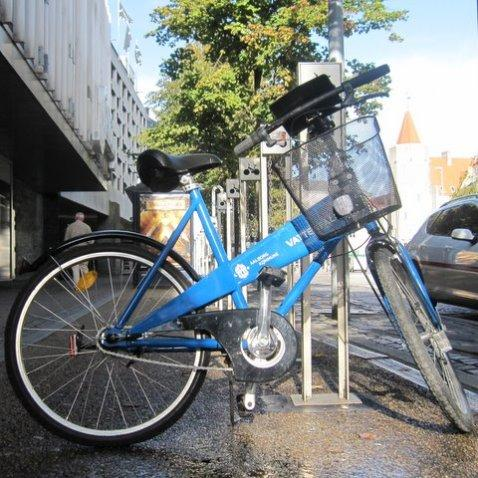
\includegraphics[width=\textwidth]{graphics/acb_bike}
\caption{An Aalborg City Bike (aalborgbycyklen.dk)}
\end{figure}
\end{column}
\end{columns}
\end{frame}
%NOTE mention interview and that it provided hardly anything new besides this

% % % % % %
% Aalborg City Bike facts
% % % % % %
\begin{frame}
\frametitle{Aalborg City Bike facts}
\begin{columns}
\begin{column}{.44\textwidth}
\begin{itemize}
\item 200 bikes
\begin{itemize}
\item 140 active
\end{itemize}
\item 21 bike stations
\begin{itemize}
\item Room for 170 bikes
\end{itemize}
\item Each bike has a lock, attached to a station
\item Unlock with 20 DKK coin, re-locking returns the coin
\end{itemize}
\end{column}
\begin{column}{.44\textwidth}
\begin{figure}
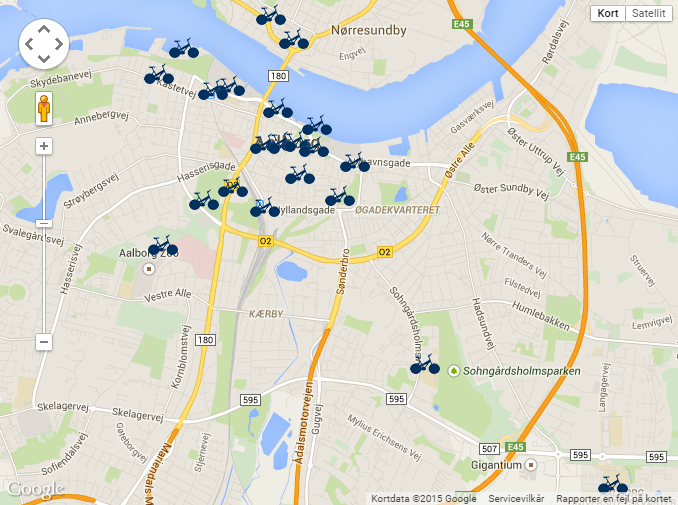
\includegraphics[width=\textwidth]{graphics/acb_gmaps}
\caption{Map of all bike stations in Aalborg/Nørresundby Area (aalborgbycyklen.dk)}
\end{figure}
\end{column}
\end{columns}
\end{frame}

% % % % % %
% Analysis summary
% % % % % %
\begin{frame}
\frametitle{Analysis summary}
\begin{columns}
\begin{column}{.45\textwidth}
\begin{block}{Problems}
\begin{enumerate}
\item Bikes left outside stations
\item Too few stations
\item Making short stops
\item No bikes at station
\item No way of knowing when a bike will arrive
\item Broken bikes
\end{enumerate}
\end{block}
\end{column}
\begin{column}{.45\textwidth}
\begin{block}{Limitations/requests}
\begin{enumerate}
\item No renting/booking system
\item No specific target user group
\item Interested in statistics about usage
\item Short period usage
\end{enumerate}
\end{block}
\end{column}
\end{columns}
\end{frame}
%NOTE mention interview with regards to limitations/requests

\subsection{Problem statement}

% % % % % %
% Trivially solved
% % % % % %
\begin{frame}
\frametitle{Trivially solved}
\begin{block}{Problems}
\begin{enumerate}
\item<1> Bikes left outside stations
\item<1> Too few stations
\item<1> Making short stops
\item<1> No bikes at station
\item<2> No way of knowing when a bike will arrive
\item<1> Broken bikes
\end{enumerate}
\end{block}
\end{frame}
%NOTE transition graying out changes between all-5 and 5

% % % % % %
% New problems
% % % % % %
\begin{frame}
\frametitle{New problems}
\begin{itemize}
\item Defining and identifying hotspots
\item Modelling the usage and using the model for predictions
\item Making the data available through a web service
\end{itemize}
\end{frame}
%NOTE sub-points with more details about the problems

% % % % % %
% Solution
% % % % % %
\begin{frame}
\frametitle{Solution}

\centering
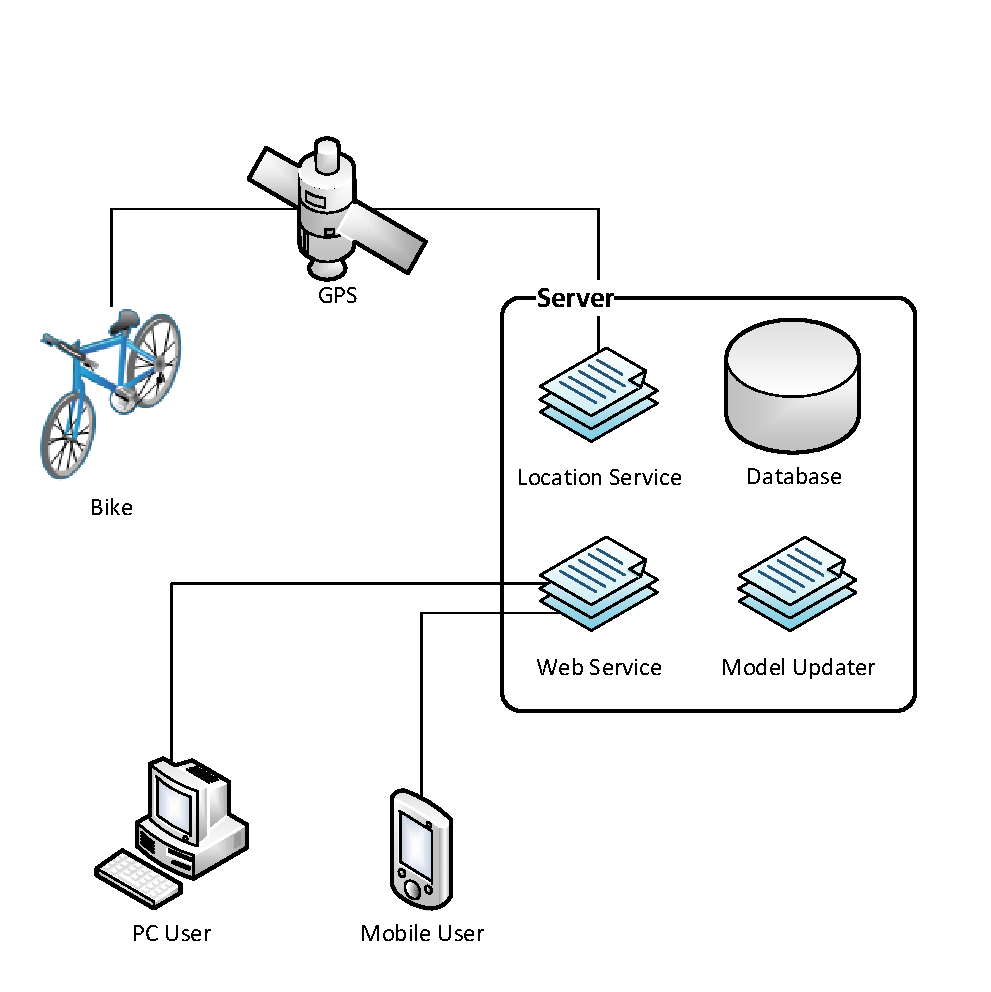
\includegraphics[height=.9\textheight]{our_solution.pdf}

\end{frame}
%NOTE think about points to add